% \documentclass[notes]{beamer}
\documentclass{beamer}
\usepackage{appendixnumberbeamer}

\usepackage{bussproofs}
\def\proofvdots#1{
    \let\tmpvskip=\extraVskip
    \def\extraVskip{-2pt}
    \noLine
    \UnaryInfC{{$\raisebox{6pt}\vdots$}}
    \noLine
    #1
    \let\extraVskip=\tmpvskip
}

\newcommand\tabdivider{\;\bigl|\;}
\newcommand\tabT[1]{\ensuremath{#1^T}}
\newcommand\tabF[1]{\ensuremath{#1^F}}

\usepackage{tikz}
\usetikzlibrary{mmt}
\usepackage{listings}
\usepackage{lstmmt}

\def\superzero{$^F$}

\makeatletter
\lst@AddToHook{OnEmptyLine}{\vspace{-0.8em}}
\makeatother

\def\highlightcolor{orange}

% \lstdefinestyle{MMT}{basicstyle=\color{black!40!blue}}

\def\elpicolor{\color{black!60!green}}
\def\elpicolorpale{\color{black!60!green!30}}

\lstdefinelanguage{ELPI}{
    morekeywords={
        kind, type, accumulate,
        prop, int, pi, sigma, is
    },
    basicstyle=\elpicolor,
    keywords=[2]{A,B,C,D,E,F,G,H,I,J,K,L,M,N,O,P,Q,R,S,T,U,V,W,X,Y,Z,X0,X1,X2,X3,X4,X5,X6,X7,X8,X9,N1,C1,C2},
    keywordstyle=[2]\itshape,
    morecomment=[l]{\%},
    morecomment=[s]{/*}{*/},
    commentstyle=\color{green!50!black!40}\itshape,
    morestring=[b]",
    showstringspaces=false,
    literate={*1}{\color{\highlightcolor}}{1} {*2}{\elpicolor}{1} {*3}{\elpicolorpale}{1},
    % morecomment=[2][s]{*1}{*2},
    % commentstyle=[2]{\color{blue}},
    % stringstyle=\color{blue},
}

% \lstset{commentstyle=\itshape\color{gray},columns=fullflexible}
\lstset{columns=fullflexible}

\usetheme{Pittsburgh}
\setbeamertemplate{footline}[frame number]
\setbeamertemplate{navigation symbols}{}
\usecolortheme{beaver}
\setbeamertemplate{frametitle}[default][left]
\setbeamertemplate{blocks}[rounded]
\setbeamercolor{block body}{bg=black!5}
\setbeamercolor{block title}{bg=black!10,fg=black}
\newcommand{\com}[1]{\strut\hfil\strut\null\nobreak\hfill\hbox{{\itshape \color{black!50}#1}}\par}

% \title{Logic-Independent Proof Search in Logical Frameworks (short paper)\footnote{\tiny The authors gratefully acknowledge project support by German Research Council (DFG) grants KO 2428/13-1 and RA-1872/3-1 OAF as well as EU Horizon 2020 grant ERI 676541 OpenDreamKit.}}
\title{Logic-Independent Proof Search in Logical Frameworks (short paper)}

\author{Michael Kohlhase\inst1 \and Florian Rabe\inst1 \and Claudio Sacerdoti Coen\inst2 \and \textbf{Jan Frederik Schaefer\inst1}}
% \institute{\inst1Computer Science, FAU Erlangen-N\"urnberg \and \inst2Department of Computer Science and Engineering, Universit\`a di Bologna}
\institute{\inst1 FAU Erlangen-N\"urnberg \and \inst2 Universit\`a di Bologna}
\date{\textbf{IJCAR} \\ remotely from Erlangen, Germany\\July 2, 2020}

\begin{document}

\begin{frame}
\titlepage
\end{frame}

\begin{frame}
    \frametitle{Logic development in MMT/LF}
    \begin{itemize}
        \item Logical frameworks can be used to describe logics
        \item We have a tool for this: MMT \com{others exist} % {\itshape\color{black!50} (others exist)}
            \begin{itemize}
                \item[$\rightarrow$] Large modular collection of logics \com{LATIN project}
            \end{itemize}
        \item Free proof checking
        \item Wouldn't it be nice to also generate provers?
        \item We report on an experiment in this direction
    \end{itemize}

    \vspace{1.5em}
    \begin{minipage}[t][2.5cm][c]{\textwidth}
    \centering
        % \only<2> {
        %     \resizebox{0.7\textwidth}{!}{\begin{tikzpicture}
        %             \node[thy,inner sep=2pt] (plsyntax) at (0, 0) {PLSyntax};
        %             \node[thy,inner sep=2pt] (plnatded) at (2.5, 0) {PLNatDed};
        %             \node[thy,inner sep=2pt] (folsyntax) at (0, -1) {FOLSyntax};
        %             \node[thy,inner sep=2pt] (folnatded) at (2.5, -1) {FOLNatDed};
        %             \node[thy,inner sep=2pt] (plhilbertpf) at (-2.5, 0) {PLHilbertPf};
        %             \node[thy,inner sep=2pt] (pdlminimalsyntax) at (3.5,1.5) {PDLMinimalSyntax};
        %             \node[thy,inner sep=2pt] (pdlaxioms) at (0, 2) {PDLAxioms};
        %             \node[thy,inner sep=2pt] (pdlrules) at (0, 1) {PDLRules};
        %             \node[thy,inner sep=2pt] (pdlpf) at (-2.5, 1.5) {PDLPf};
        %             \node[thy,inner sep=2pt] (plnatdedclassical) at (6,0) {PLNatDedClassical};
        %             \node[thy,inner sep=2pt] (sfolsyntax) at (-2.5, -1) {SFOLSyntax};
        %             \draw[include] (plsyntax) -- (plnatded);
        %             \draw[include] (plsyntax) -- (folsyntax);
        %             \draw[include] (plsyntax) -- (sfolsyntax);
        %             \draw[include] (plsyntax) -- (plhilbertpf);
        %             \draw[include] (plsyntax) -- (pdlminimalsyntax);
        %             \draw[include] (folsyntax) -- (folnatded);
        %             \draw[include] (plnatded) -- (folnatded);
        %             \draw[include] (plnatded) -- (plnatdedclassical);
        %             \draw[include] (plhilbertpf) -- (pdlpf);
        %             \draw[include] (pdlaxioms) -- (pdlpf);
        %             \draw[include] (pdlrules) -- (pdlpf);
        %             \draw[include] (pdlminimalsyntax) -- (pdlaxioms);
        %             \draw[include] (pdlminimalsyntax) -- (pdlrules);
        %     \end{tikzpicture}}
        % }
        % \only<3> {
        %     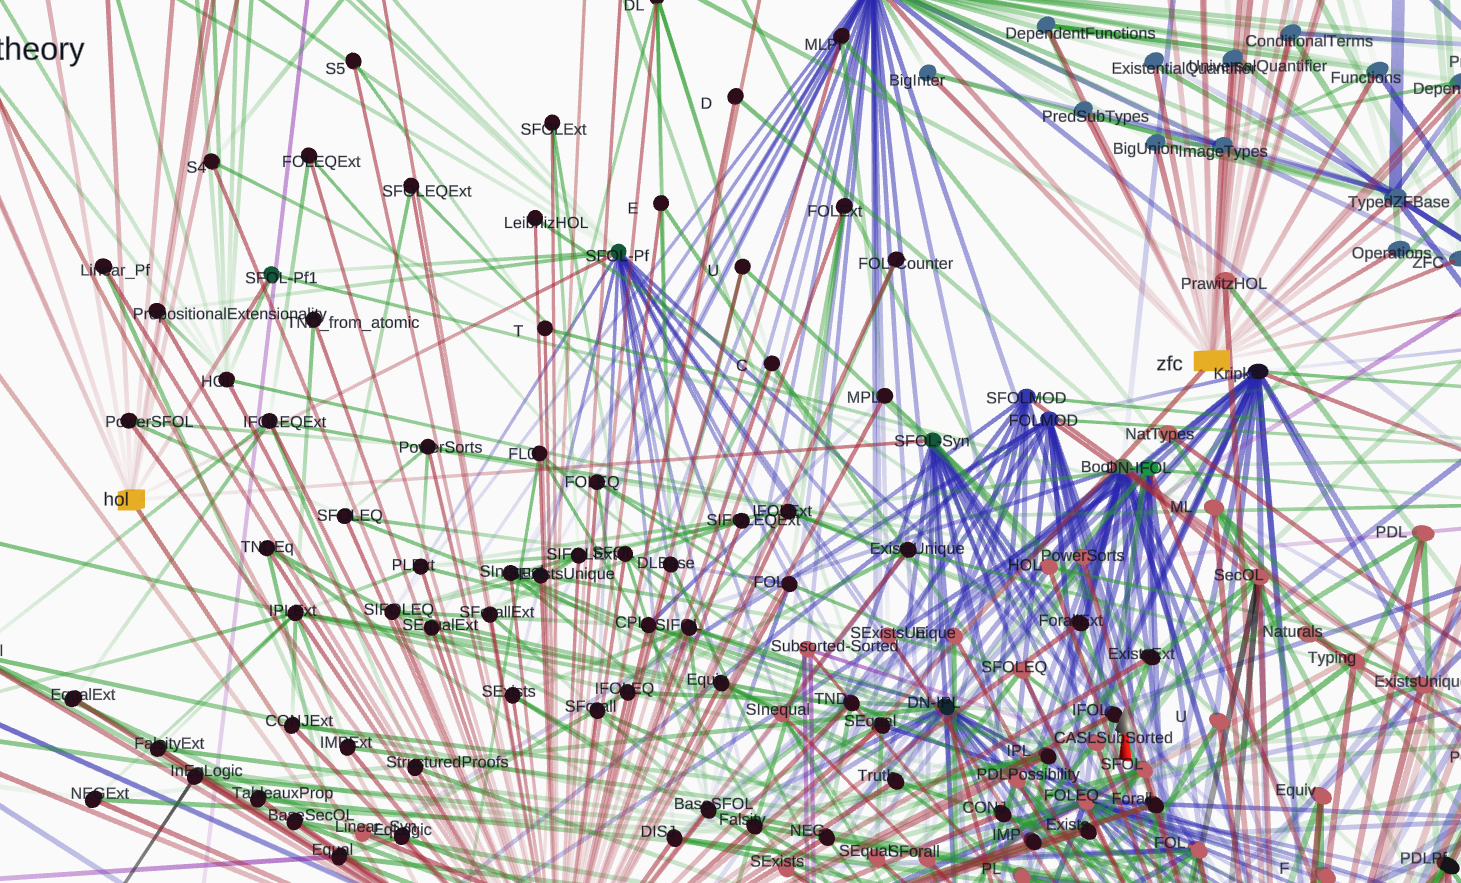
\includegraphics[scale=0.1]{latinclose.png}
        % }
        % \only<4> {
        %     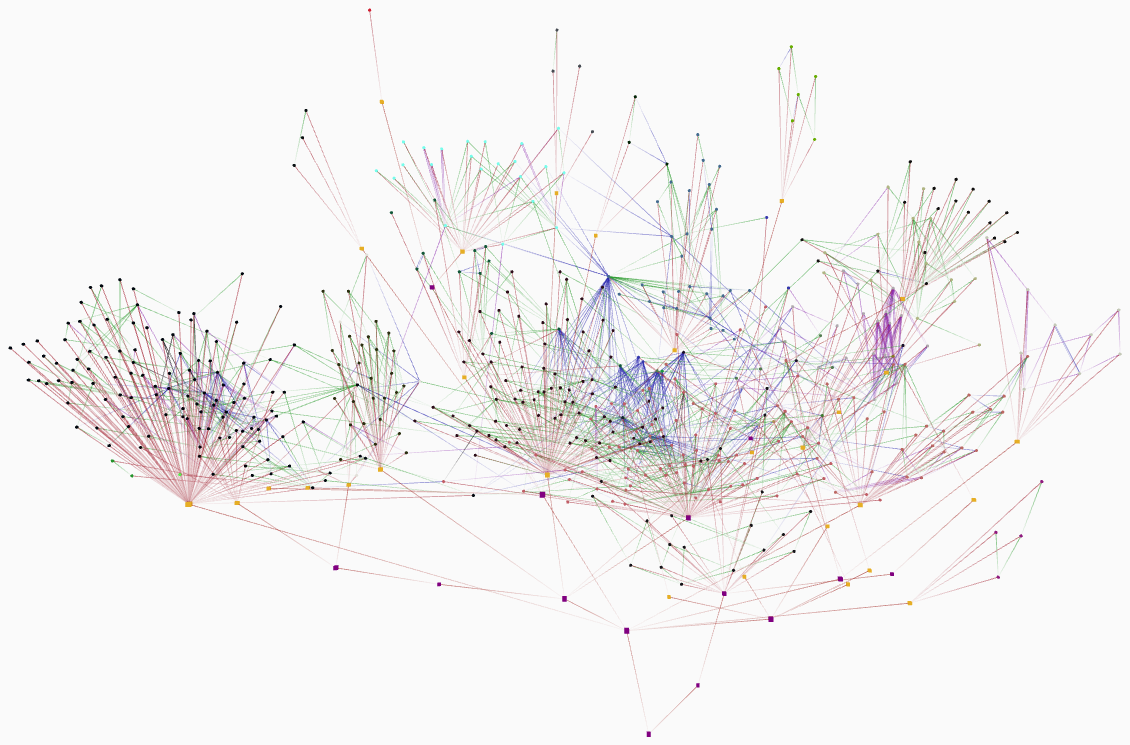
\includegraphics[scale=0.13]{latinfar.png}
        % }
        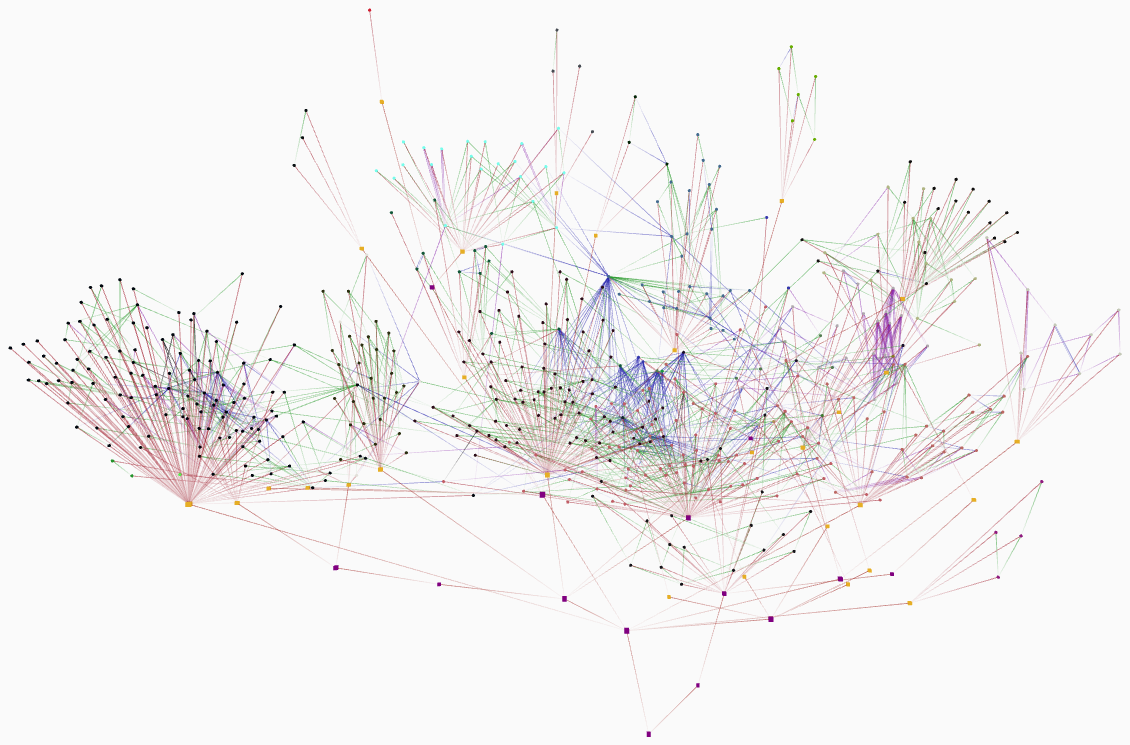
\includegraphics[scale=0.13]{latinfar.png}
    \end{minipage}
\end{frame}

% \begin{frame}
%     \frametitle{Logic-Independent Proof Search in Logical Frameworks}
%     \begin{itemize}
%         \item Logical frameworks like LF allow us to describe logics
%         \item You get: proof checking
%         \item Wouldn't it be nice to also generate provers?
%         \item We report on an experiment in this direction
%     \end{itemize}
% \end{frame}
% 
% \note{
%     Logical frameworks like LF can be used to describe different logics.
%     Apart from the syntax you can also describe calculi.
%     That means that you get proof checking basically for free
%     because it's nothing else than type checking.
%     However, you still have to write the proofs somehow,
%     and that can be a lot of work.
%     So wouldn't it be nice if we could simply generate automated theorem provers from the logic we specified?
%     Even if they are not very efficient, it could help us a lot.
%     So we did some experiments in that direction
%     and I would like to report on that.
% }
% 
% \begin{frame}
%     \frametitle{Logic Development in MMT}
%     \begin{minipage}{0.6\textwidth}
%         \begin{itemize}
%             \item knowledge represented in theories
%             \item theories linked by morphisms
%             \item different meta levels
%             \item MMT is foundation-independent
%             \item we will restrict ourselves to LF
%         \end{itemize}
%     \end{minipage}\hfill
%     \begin{minipage}{0.39\textwidth}
%         \centering
%         \begin{tikzpicture}[xscale=0.9]
%             \onslide<2>{\draw[color=blue,fill=blue!20,rounded corners=0.1cm] (-2.0,2.0) rectangle (1.9,1.0);}
%             \node[thy] (lf) at (0,2.5)  {$\mathsf{LF}$};
%             \node[thy] (lfx) at (-1.8,2.5)  {$\mathsf{LF+X}$};
%             \node[thy] (fol) at (-1,1.5)   {$\mathsf{FOL}$};
%             \node[thy] (hol) at (.9,1.5) {$\mathsf{HOL}$};
%             \node[thy] (mon) at (-2.5,0) {$\mathsf{Monoid}$};
%             \node[thy] (gp) at (-.5,0) {$\mathsf{CGroup}$};
%             \node[thy] (rg) at (1.5,0)  {$\mathsf{Ring}$};
%             % \node[thy] (zfc) at (-2.8,1) {$\mathsf{ZFC}$};
%             \draw[meta](lf) -- (fol);
%             \draw[meta](lf) -- (hol);
%             \draw[meta](fol) -- (mon);
%             \draw[meta](fol) -- (gp);
%             \draw[meta](hol) -- (rg);
%             \draw[include](lf) -- (lfx);
%             % \draw[view](fol) -- node[above] {\footnotesize$\mathsf{f2h}$} (hol);
%             \draw[view] (fol) -- (hol);
%             \draw[struct](gp) to[bend right=10] node[below] {\footnotesize$\mathsf{add}$} (rg);
%             \draw[struct](mon) to[out=20,in=160] node[above] {\footnotesize$\mathsf{mult}$} (rg);
%             \draw[include](mon) -- (gp);
%             % \draw[meta] (fol) -- (zfc); %$
%             % \draw[view] (fol)  to[bend right=30] node[above,near start]{\footnotesize$\mathsf{folsem}$} (zfc); %$
%             % \draw[view] (mon) -- node[left]{\footnotesize$\mathsf{mod}$} (zfc); %$
%         \end{tikzpicture}
%     \end{minipage}
% 
% %     \vspace{2em}
% %     % \onslide<2>\textbf{Outline:\\We can specify logics in MMT.\\ How can we generate provers?}
% %     \centering
% %     \onslide<2>\textbf{We can specify logics in MMT.}
% % 
% %     \onslide<2>\textbf{How can we generate provers?}
% %     \vspace{2em}
% \end{frame}

\begin{frame}[fragile]
    \frametitle{Logic Syntax in MMT/LF}
    \begin{minipage}{0.7\textwidth}
        \begin{lstlisting}[language=MMT]
theory PropLog =
    prop : type

    not : prop \raa prop
    and : prop \raa prop \raa prop
    or : prop \raa prop \raa prop
    ...
        \end{lstlisting}

        \begin{lstlisting}[language=MMT]
theory FOL =
    include PropLog

    term : type

    forall : (term \raa prop) \raa prop    // Higher-order abstract syntax
    exists : (term \raa prop) \raa prop
        \end{lstlisting}
    \end{minipage}
    \begin{minipage}{0.1\textwidth}
        \begin{tikzpicture}
            \node[thy,inner sep=3pt] (pl) at (0,0) {PropLog};
            \node[thy,inner sep=3pt] (fol) at (0, -2) {FOL};
            \draw[include] (pl) -- (fol);
        \end{tikzpicture}
    \end{minipage}
\end{frame}

\begin{frame}[fragile]
    \frametitle{Natural Deduction in MMT/LF}
    \begin{minipage}{0.9\textwidth}
        \centering
        \begin{minipage}{0.49\textwidth}
            \begin{prooftree}
                \AxiomC{$A \wedge B$}
                \RightLabel{\lstinline|andEl|}
                \UnaryInfC{$A$}
            \end{prooftree}
        \end{minipage}
        \begin{minipage}{0.49\textwidth}
            \begin{prooftree}
                \def\defaultHypSeparation{\hskip 0pt}
                \AxiomC{$A \vee B$}
                \AxiomC{$\,\,[A]^1$}
                \proofvdots{\UnaryInfC{$C$}}
                \AxiomC{$\,\,[B]^1$}
                \proofvdots{\UnaryInfC{$C$}}
                \RightLabel{\lstinline|orE|$^1$}
                \TrinaryInfC{$C$}
            \end{prooftree}
        \end{minipage}
    \end{minipage}

    \vspace{1.5em}
    \begin{lstlisting}[language=MMT]
theory PropLog_ND =
    include PropLog

    // ded X is type of proofs for X  (judgments as types)
    ded : prop \raa type


    andEl : {A,B} ded (and A B) \raa ded A

    orE : {A,B,C} ded (or A B) \raa (ded A \raa ded C) \raa
                      (ded B \raa ded C) \raa ded C
    \end{lstlisting}
\end{frame}

\begin{frame}[fragile]
    \frametitle{Generating Provers in ELPI}
    \begin{itemize}
        \item ELPI is an extension of $\lambda$Prolog \com{$\approx$ Prolog + HOAS}\note{ELPI was developed by Claudio and others}
        \item Optimized for fast execution of logical algorithms \com{type inference, unification, proof search, \dots}
    \end{itemize}

    \vspace{2em}
    
    \makebox[2.5cm][l]{\textbf{LF rule}} \lstinline[language=MMT]|andEl : {A,B} ded (and A B) \raa ded A|

    \vspace{1.0em}
    \textbf{ELPI equivalent}

    \vspace{0.5em}
    \makebox[2.5cm][r]{direct:$\;\;$} \lstinline[language=ELPI]|pi A \ pi B \ ded (and A B) => ded A.|

    \vspace{0.5em}
    \makebox[2.5cm][r]{syn. sugar:$\;\;$} \lstinline[language=ELPI]|ded A :- ded (and A B).|

\end{frame}

\begin{frame}[fragile]
    \frametitle{From LF to ELPI}
    % \textbf{Or-elimination}

    \begin{block}{{\bfseries Example:} Or-Elimination}
    \vspace{0.5em}
    \makebox[1cm][l]{LF:}\begin{minipage}{0.85\textwidth}
        \lstinline[keepspaces=true,language=MMT]|orE : {A,B,C} ded (or A B) \raa (ded A \raa ded C) \raa|
        \lstinline[keepspaces=true,language=MMT]|                 (ded B \raa ded C) \raa ded C|
    \end{minipage}

    \vspace{1em}
    \makebox[1cm][l]{ELPI:}\lstinline[language=ELPI,keepspaces=true]|ded C :- ded (or A B), ded A => ded C, ded B => ded C.|
    \vspace{0.5em}
    \end{block}

    \vspace{1em}

    \begin{block}{{\bfseries Example:} Forall-Introduction}
    % \textbf{Forall-introduction}
    \vspace{0.5em}
    \makebox[1cm][l]{LF:}\begin{minipage}{0.85\textwidth}
        \lstinline[keepspaces=true,language=MMT]|forallI : {P} ({x} ded (P x)) \raa ded (forall P)|
    \end{minipage}

    \vspace{1em}
    \makebox[1cm][l]{ELPI:}\lstinline[language=ELPI,keepspaces=true]|ded (forall P) :- pi x \ ded (P x).|
    \vspace{0.5em}
    \end{block}
\end{frame}

\begin{frame}[fragile]
    \frametitle{Controlling the Proof Search}
    \begin{itemize}
        \item Problem: Search diverges \com{searching harder than checking}
        \item Solution: Control search with helper predicates:
            \com{inspired by ProofCert project by Miller et al.}\note{ProofCert assumes a focused logic, we don't}
            % \\{ \itshape\color{black!50}\makebox[10cm][r]{(inspired by ProofCert project by Miller et al.)}}
            \begin{itemize}
                \item Intuition: Decide whether to apply rule
                \item Do not affect correctness
                \item Extra argument tracks aspects of proof state
            \end{itemize}
    \end{itemize}

    \vspace{1.5em}
    \makebox[1.2cm][l]{Before:} {\def\highlightcolor{white}\makebox[5.7cm][l]{\lstinline[language=ELPI]|ded *1X *2A :-|}\lstinline[language=ELPI]|*2ded *1X1 *2(and A B).|}

%     \vspace{0.5em}
%     \makebox[1.2cm][l]{Depth-limit:} \makebox[5.7cm][l]{\lstinline[language=ELPI,keepspaces=true]|ded *1X *2A :- *1X > 0, X1 is X-1,*2|}\lstinline[language=ELPI,keepspaces=true]|ded *1X1 *2(and A B).|

    \vspace{0.5em}
    \makebox[1.2cm][l]{Now:} \makebox[5.7cm][l]{\lstinline[language=ELPI]|ded *1X *2A :- *1help/andEl X A B X1,*2|}\lstinline[language=ELPI]|ded *1X1 *2(and A B).|

%     \vspace{2.0em}
%     Example helper for depth-limit:
% 
%     \vspace{0.5em}
%     \lstinline[language=ELPI,keepspaces=true]|    help/andEl (idcert N) _ _ (idcert N1) :- N > 0, N1 is N - 1.|
\end{frame}

\begin{frame}[fragile]
    \frametitle{Helper Predicates}
        \renewcommand{\arraystretch}{1.5}
    \begin{tabular}{l p{3.5cm} p{3.5cm}}
        \textbf{Name} & \textbf{Predicate} & \textbf{Argument} \\
        Iter. deepening & checks depth & remaining depth \\
        Proof term & generates term & proof term \\
        Product & calls other predicates & arguments for other predicates \\
        Backchaining &
            \footnotesize Prolog's backchaining ($\approx$ forward reasoning from axioms via $\Rightarrow$/$\forall$ elimination rules) &
            \footnotesize pattern of formula to be proven (e.g. a conjunction) \\
        % Backchaining & \multicolumn2{p{7cm}}{\footnotesize Restricts new formulae in e.g. elimination rules to those that could be proven by forward reasoning} \\
    \end{tabular}

    \vspace{1.5em}
    \begin{block}{\textbf{Example helper:} Iterative deepening}
        \lstinline[language=ELPI,keepspaces=true]|help/andEl (idcert N) _ _ (idcert N1) :- N > 0, N1 is N - 1.|
    \end{block}

%     Example call:
%     \begin{lstlisting}[language=ELPI]
%     ?- ded (prodcert (idcert 2) (ptcert Proof)) (impl a (or a b)).
% 
%     Proof = implI a (or a b) (orIl a b (i a)).
%     \end{lstlisting}
\end{frame}

\begin{frame}[fragile]
    \frametitle{Tableau Provers}
    \note{We can scale in terms of logics supported or (orthogonally) in terms of prover strategies.
    We went for the latter.}
    \begin{minipage}[b][2cm][b]{0.4\textwidth}
        \begin{prooftree}
            \AxiomC{$\;\tabF{A \wedge B}$}
            \RightLabel{andF}
            \UnaryInfC{$\tabF{A} \tabdivider \tabF{B}$}
        \end{prooftree}
    \end{minipage}
    \begin{minipage}[b][2cm][b]{0.4\textwidth}
        \def\defaultHypSeparation{\hskip 0pt}
        \begin{prooftree}
            \AxiomC{$\tabF{A \wedge B}$}
            \AxiomC{$\;[\tabF{A}]$}
            \proofvdots{\UnaryInfC{$\bot$}}
            \AxiomC{$\;[\tabF{B}]$}
            \proofvdots{\UnaryInfC{$\bot$}}
            \RightLabel{andF}
            \TrinaryInfC{$\bot$}
        \end{prooftree}
    \end{minipage}

    \vspace{2em}
    \makebox[1.0cm][l]{LF:} \lstinline[language=MMT]|andF : {A,B} A\wedgeB\super0 \raa (A\super0 \raa \bot) \raa (B\super0 \raa \bot) \raa \bot|

    \vspace{0.5em}
    \makebox[1.0cm][l]{ELPI:} \lstinline[language=ELPI]|closed *3X *2:- *3help/andF X A B X1 X2 X3, *2f *3X1 *2(and A B),|
    \lstinline[language=ELPI,keepspaces=true]|                         f*3/hyp *2A => closed *3X2*2, f*3/hyp*2 B => closed *3X3*2.|

    \vspace{2em}
    With iterative deepening we get a working prover!

    $\rightarrow$ Other helpers result in more efficient provers
\end{frame}

    
\begin{frame}[fragile]
    \frametitle{Conclusion}
    Summary:

    \begin{itemize}
        \item Develop logic in MMT/LF \note{MMT has mechanisms for checking the soundness of calculi, which translates into soundness of the generated provers}
        \item Generate ELPI provers from specified calculi
        \item Soundness w.r.t. MMT specification for free
        \item Can show soundness of calculus in MMT
    \end{itemize}

    \vspace{1em}
    Goals:
    \begin{itemize}
        \item Help logic developers with provers \com{MMT users}
        \item Help prover makers test strategies across logics \com{ELPI users}
    \end{itemize}

    \vspace{1em}
    Evaluation:
    \begin{itemize}
        \item Experiment at an early stage \com{more logics, strategies}
        \item Translation to FOL probably often more efficient \note{Advantage over translation to FOL: we directly get proof terms}
        \item Test run: { \footnotesize
            \begin{tabular}{l l l}
                Generated (ND) & Me & Vampire\\
                1.007 s (depth 9) & $\approx$ 16 min & 0.001s
            \end{tabular}
        }
    \end{itemize}

%     \vspace{1.5em}
%     \makebox[1.5cm][l]{MMT/LF:} \lstinline[language=MMT]|andEl : {A,B} ded (and A B) \raa ded A|
%     
%     \vspace{0.5em}
%     \makebox[1.5cm][l]{ELPI:} \lstinline[language=ELPI]|ded *1X *2A :- *1help/andEl X A B X1*2, ded *1X1 *2(and A B).|

%     \vspace{0.5em}
%     \makebox[1.3cm][l]{Helper:} \lstinline[language=ELPI]|help/andEl (idcert N) _ _ (idcert N1) :- N > 0, N1 is N - 1.|
\end{frame}

\appendix

\begin{frame}
    \frametitle{Bonus: Soundness and Completeness in MMT}
    \centering

    \begin{tikzpicture}[xscale=1]
        \node[thy] (pl) at (0,0) {PropLog};
        \node[thy,black!60] (fol) at (2.5,0) {FOL};
        \node[thy] (nd) at (-1.5,-1.5) {ND};
        \node[thy] (tab) at (1.5,-1.5) {Tableau};
        \draw[include,black!60] (pl) -- (fol);
        \draw[include] (pl) -- (nd);
        \draw[include] (pl) -- (tab);
        \draw[view] (nd) to[bend left=15] (tab);
        \draw[view] (tab) to[bend left=15] (nd);
    \end{tikzpicture}

    \vspace{2em}
    \begin{itemize}
        \item Express ND rules in terms of tableau rules
        \item Express tableau rules in terms of ND rules
        \item $\leadsto$ ND and tableau calculus can prove same set of propositions
        \item $\leadsto$ ND sound and complete $\Leftrightarrow$ tableau sound and complete
        % \item Generated provers sound, not necessarily complete
    \end{itemize}
\end{frame}

\begin{frame}[fragile]
    \frametitle{Bonus: Helper Predicates in ELPI (as they are generated)}
    \begin{lstlisting}[language=ELPI]
% iterative deepening
help/andEl (idcert X3) A B (idcert X2) :- X3 > 0 , X2 is X3 - 1.


% record proof terms
help/andEl (ptcert (andEl A B X2)) A B (ptcert X2).


% combine helpers
help/andEl (prodcert X3/1 X3/2) A B (prodcert X2/1 X2/2) :-
   help/andEl X3/1 A B X2/1 , help/andEl X3/2 A B X2/2.


% back-chaining
help/andEl (bccert X3) A B (bccert (bc/fwdLocked X2)) :-
   bc/val X3 X4 , X4 > 0 , X2 is X4 - 1 , bc/fwdable (and A B).
    \end{lstlisting}
\end{frame}

\end{document}
